\documentclass[a4paper, 12pt]{article}
\usepackage[T2A,T1]{fontenc}
\usepackage[utf8]{inputenc}
\usepackage[english, russian]{babel}
\usepackage{graphicx}
\usepackage[hcentering, bindingoffset = 10mm, right = 13 mm, left = 13 mm, top=20mm, bottom = 20 mm]{geometry}
\usepackage{multirow}
\usepackage{lipsum}
\usepackage{amsmath, amstext}
\usepackage{siunitx}
\usepackage{mathrsfs}
\usepackage{subcaption}
\usepackage{wrapfig}
\usepackage{adjustbox}
\usepackage{enumerate, indentfirst, float}
\usepackage{capt-of, svg}
\usepackage{icomma}
\usepackage{pgfplots}
\usepackage{xcolor}
\usepackage{hyperref}
\newenvironment{bottompar}{\par\vspace*{\fill}}{\clearpage}
\definecolor{linkcolor}{HTML}{799B03} % цвет ссылок
\definecolor{urlcolor}{HTML}{799B03} % цвет гиперссылок

\hypersetup{pdfstartview=FitH,  linkcolor=linkcolor,urlcolor=urlcolor, colorlinks=true}
\author{Михеев Илья}
\title{ ВПВ на тему "Коронный разряд"!}
\date{\today}
\begin{document}
	
	\maketitle
	\newpage

\section{Теория}
\subsection{Определение}
Коронный разряд --- это самостоятельный газовый разряд, возникающий в резко неоднородных полях у электродов с большой кривизной поверхности (острия, тонкие провода). Зона вблизи такого электрода характеризуется значительно более высокими значениями напряженности поля по сравнению со средними значениями для всего промежутка. Когда напряжённость поля достигает предельного значения (для воздуха около 30 кВ/см), вокруг электрода возникает свечение, имеющее вид короны. При коронном разряде ионизационные процессы происходят только вблизи коронирующего электрода. Коронный разряд возникает при сравнительно высоком давлении воздуха (порядка атмосферного). 
\subsection{Механизм возникновения}
Электрон, возникший при случайной ионизации нейтральной молекулы, ускоряется в электрическом поле и приобретает энергию, достаточную для того, чтобы при столкновении со следующей молекулой ионизовать её. В результате происходит лавинное увеличение числа заряженных частиц.

Если коронирующее остриё является катодом, такую корону называют отрицательной. В отрицательной короне ионизационные лавины направлены от острия. Воспроизведение свободных электронов обеспечивается здесь за счёт термоэмиссии из коронирующего электрода. На некотором удалении от острия, там где электрическое поле является недостаточным, чтобы обеспечивать лавинную ионизацию, электроны рекомбинируют с нейтральными молекулами, образуя отрицательные ионы, которые и являются носителями тока во внешней области.

Если коронирующее остриё является анодом, такую корону называют положительной. В положительной короне электроны притягиваются к острию, а ионы отталкиваются от него. Воспроизведение электронов, запускающих ионизационную лавину, обеспечивают вторичные фотопроцессы в газе вблизи от острия. Вдали от коронирующего электрода электрическое поле является недостаточным, чтобы обеспечивать лавинную ионизацию. Носителями тока в этой области являются положительные ионы, движущиеся от острия к отрицательному электроду. В отличие от ровного свечения отрицательной короны, в положительной короне иногда наблюдаются разбегающиеся от острия стримеры, которые при увеличении напряжения превращаются в искровые каналы. 
\section{Эксперимент}
В эксперименте необходимо было создать большую разность потенциалов, я воспользовался ионизатором воздуха, сократив расстояние между катодом и анодом\\
Само получение этого разряда на видео:\\ \href{https://www.youtube.com/watch?v=vwNDfH06hh0}{https://www.youtube.com/watch?v=vwNDfH06hh0}
\begin{figure}[H]
	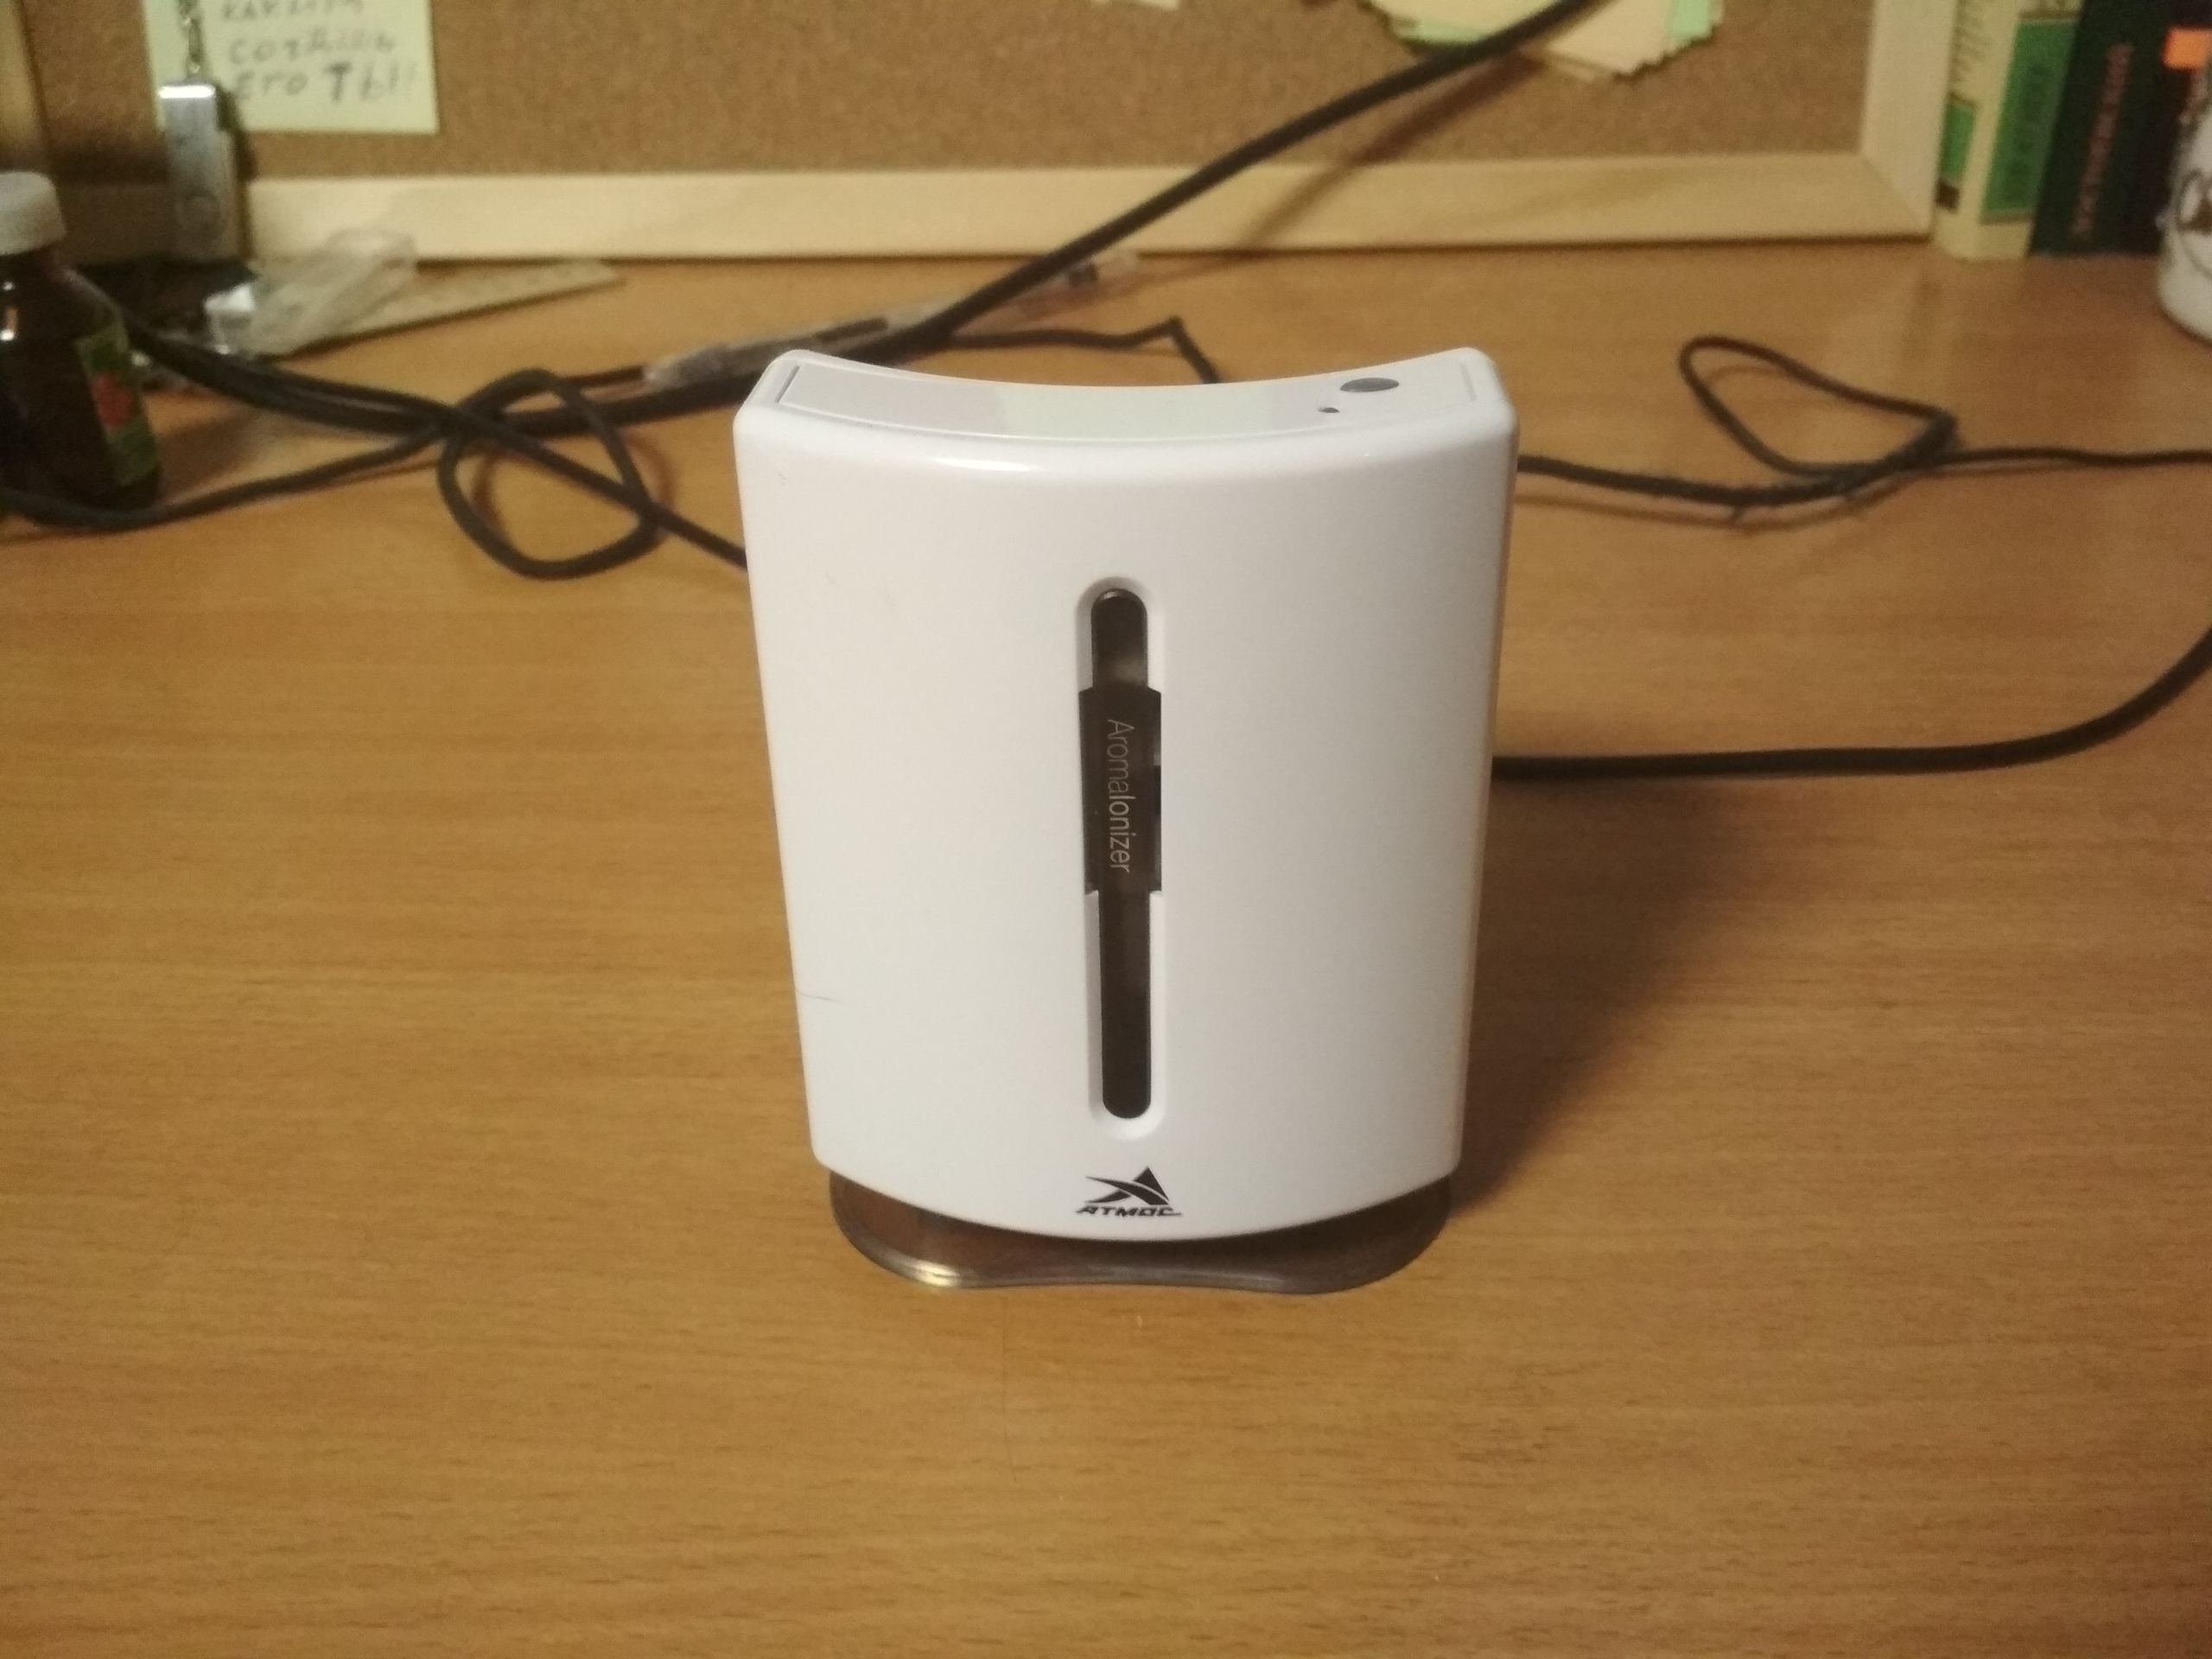
\includegraphics[width = 0.6\textwidth]{1.jpg}
\end{figure}
\begin{figure}[H]
	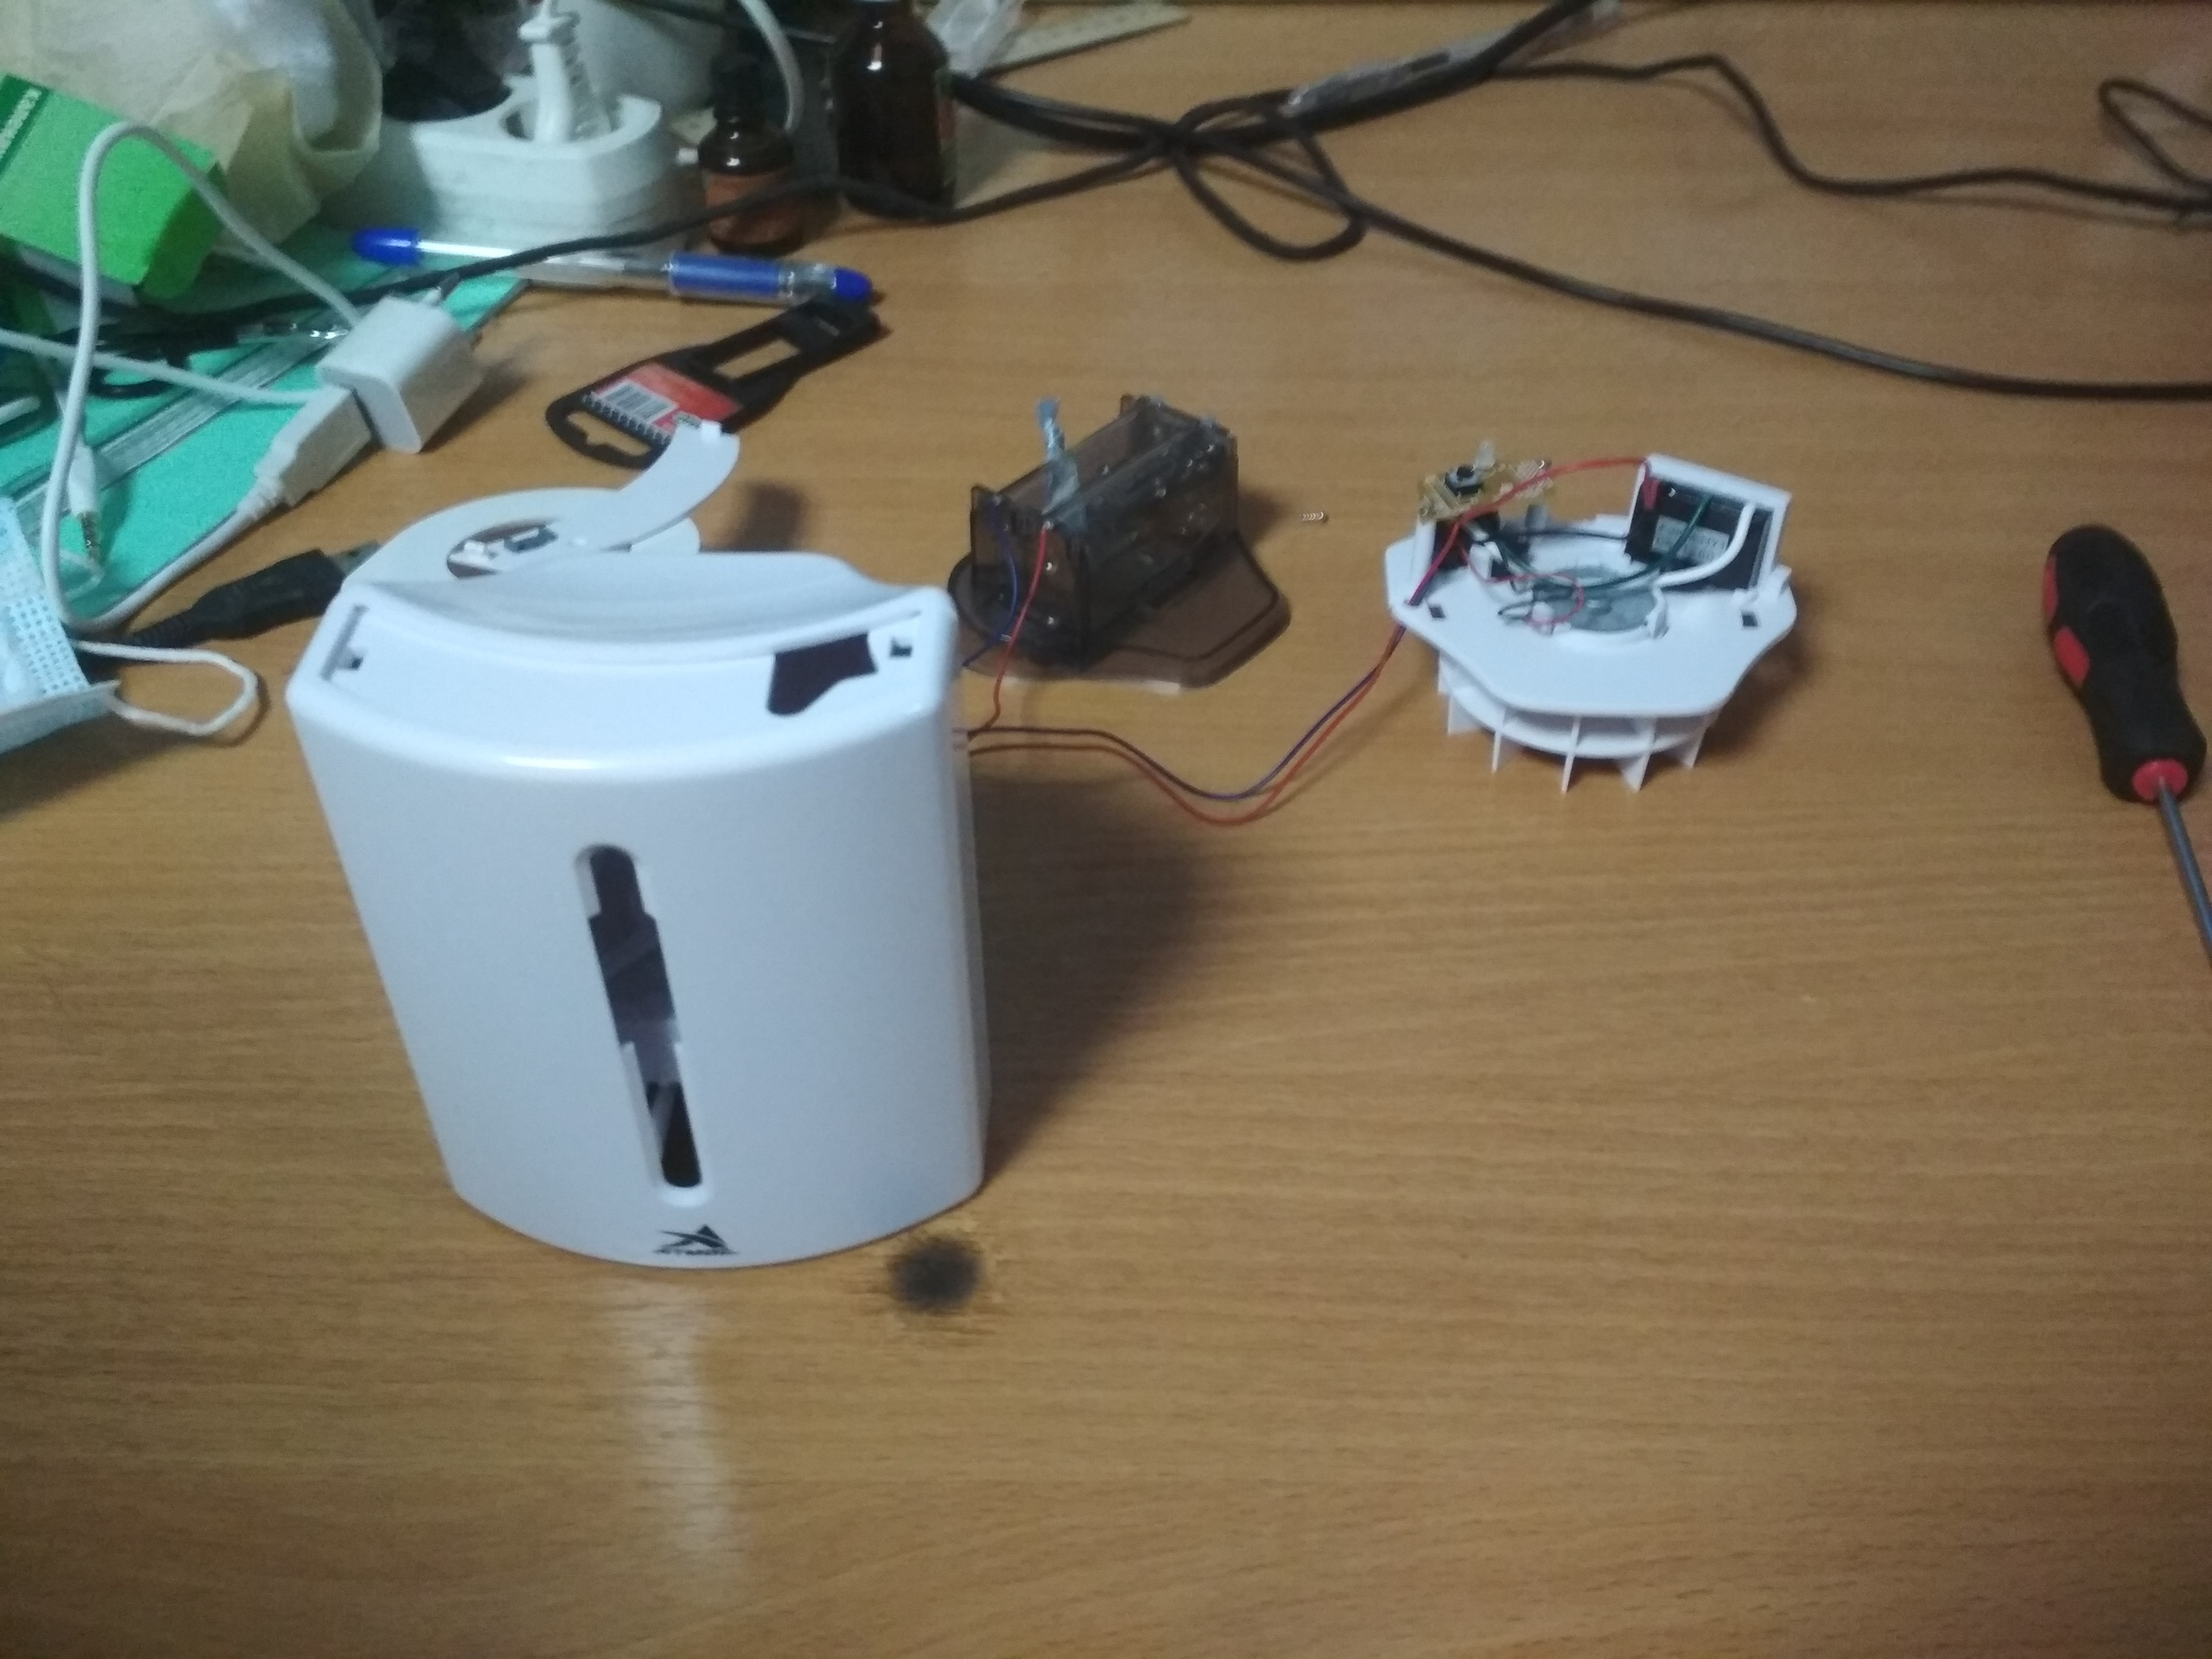
\includegraphics[width = 0.6\textwidth]{2.jpg}
\end{figure}
\begin{figure}[H]
	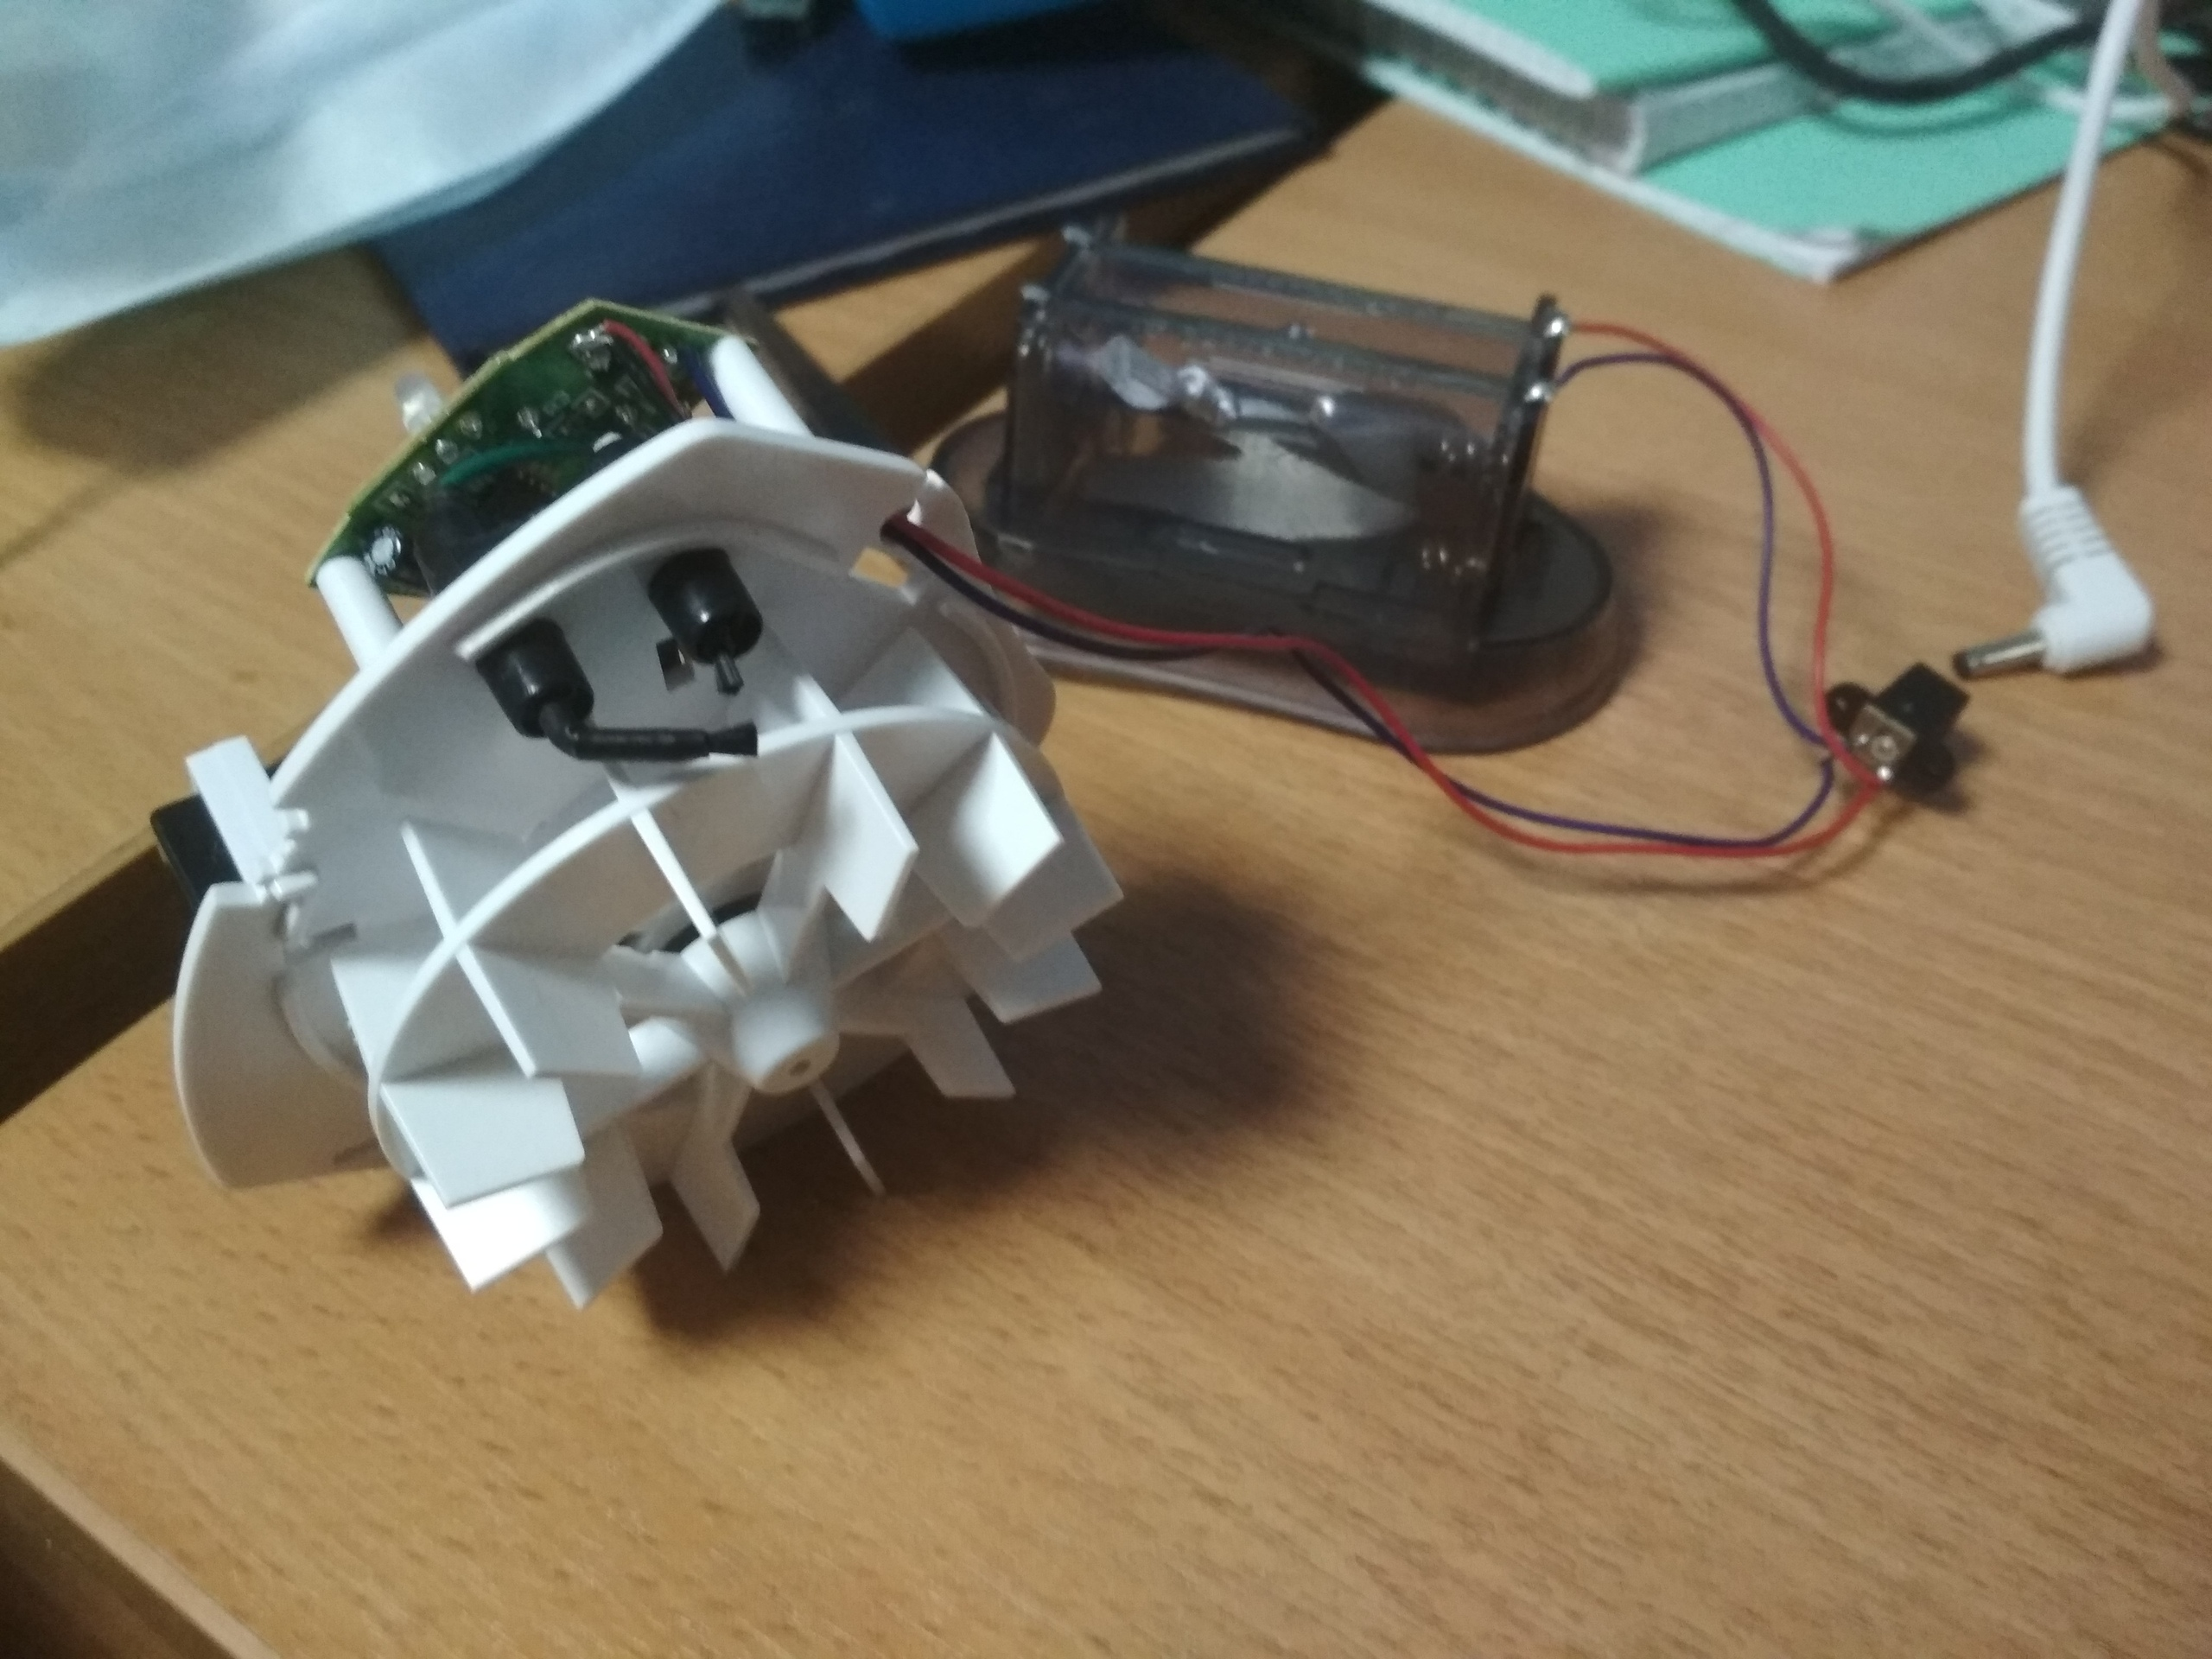
\includegraphics[width = 0.6\textwidth]{3.jpg}
\end{figure}

\end{document}